\begin{frame}[t,fragile]{量子加算器}
  \begin{itemize}
    %\setlength{\itemsep}{1em}
  \item 1量子ビットの加算 $\Rightarrow$ CCXゲートとCXゲートで実現できる
    \begin{center}
      \resizebox{0.5\textwidth}{!}{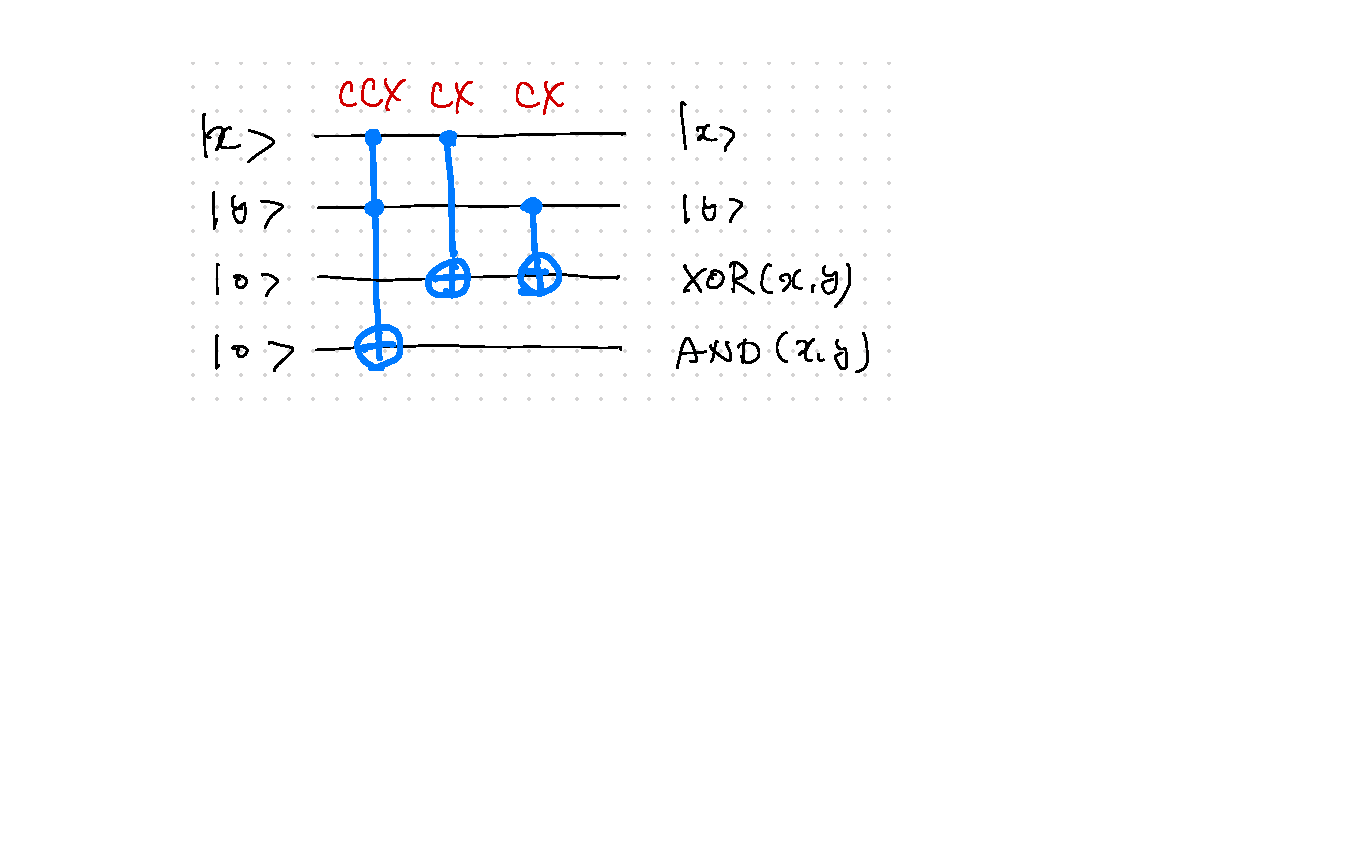
\includegraphics{image/adder1.pdf}}
    \end{center}
  \item CCXゲートは、Hゲート、Rzゲート、CXゲートの組み合わせで表現できる
  \item 任意の量子回路は、Hゲート、Rzゲート、CXゲートの組み合わせで表現できる (万能量子ゲート)
  \end{itemize}
\end{frame}
